\begin{itemize}
  \item Model-free DRL method that leverages small amount of demonstration data to assist RL agent
  \item Applied to robotic manipulation tasks, end-to-end visuomotor policies that map RGB camera inputs to joint velocities
  \item RL for robotics, policies must map multi-modal and partial information to control of many DOFs
  \item Real tasks have contact-rich dynamics and vary along many dimensions, generalization challenge
  \item Exploration is challenging due to high-dimensional and continuous action space
  \item Techniques for exploiting priviledged + task specific information to accelerate + stabilize training
  \item Combine IL with RL using a hybrid reward (imitation reward based on GAIL)
  \item Also use demonstrated data to create a curriculum by randomizing the start state distribution
  \item Learn policy and value in separate modalities
  \item Value function is used in PPO for estimating the advantage to compute policy gradient, instead of using pixels, they use low-level physical states to train value function
  \item Auxiliary tasks for visual modules
  \begin{itemize}
    \item improve learning efficiency
    \item state-prediction layer used to predict locations of objects from camera observation
    \item use fully-connected layer to regress 3D coordinates, minimize $l_{2}$ loss
  \end{itemize}
  \item GAIL discriminator uses object-centric representations (positions of objects), requires some domain knowledge
  \item Diversify training conditions such as visual appearance, object geometry, and system dynamics to sim2real transfer
  \item Deep visuomotor policy takes as input RGB observation and proprioceptive features (joint positions and angular velocities)
  \item GAIL has two networks: a policy network and a discriminator network and uses a min-max objective
  \item Policy is trained using policy gradient methods to maximum discounted sum of reward
  \item Employing shaping reward as a trick to facilitate exploration. Task rewards given as a sparse reward at different stages of the tasks, e.g. block stacking - reaching, lifting, stacking
  \item This is better than hand-crafting a dense shaping reward
  \item Hybrid reward: $r(s_{t}, a_{t}) = \lambda r_{gail}(s_{t}, a_{t}) + (1-\lambda) r_{task}(s_{t}, a_{t})$
  \item There is a balanced contribution between RL and IL rewards
  \begin{figure}[H]
    \caption{Deep Visuomotor Policy}
    \centering
    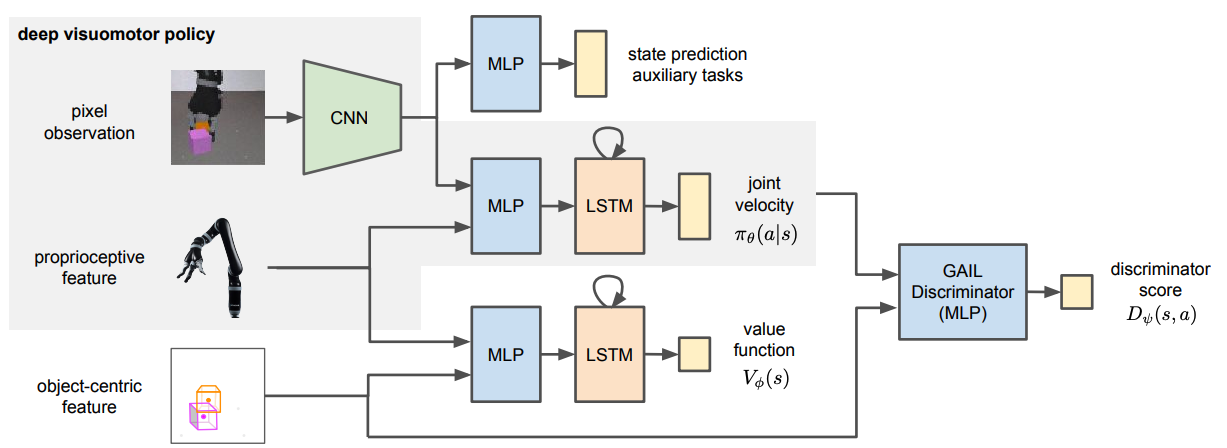
\includegraphics[width=\textwidth]{../../imgs/visuomotor_skills.png}
  \end{figure}
  \item Experiments
  \begin{itemize}
    \item Block lifting, block stacking, pouring liquid, order fulfillment, clearing table
    \item Kinova Jaco arm has 9 DOF: 6 arm joints and 3 actuated fingers
    \item Used various objects ranging from basic geometric shapes to 3D objects made from primitive shapes
    \item Sim2real is still a challenge, large domain gap, transfer is hindered by visual discrepancies, arm dynamics, and physical properties of the environment
    \item Certain level of degradation when running on a real robot, zero-shot sim2real transfer
    \item On a real robot, there is often a delay in execution of action which is detrimental to robot's performance
    \item Fine-tuned agent in simulation subjected to a random chance of dropping actions
  \end{itemize}
\end{itemize}